\section{Geometría Proyectiva}
\subsection{Contexto e idea}
Segun el programa de Erlegen, una geometría se basa en el estudio de invariantes
al aplicar unas ciertas transformaciones. Así tenemos que las geometrías estan
"incluidas" en las superiores.

Así, la geometría euclidea, que estudia las transformaciones ortogonales, estaría
"incluída" en la geometría afín, que estudia las tansformaciones lineales. Aquí
se muestra una tabla con las distintas geometrías en la cual cada una esta
"incluída" en la anterior
\begin{center}
	\begin{tabular}{|c|c|}
		\hline Geometría & Transformaciones de estudio \\
		\hline \hline
		G. euclídea  & transformaciones ortogonales \\ \hline
		G. afín & transformaciones lineales \\ \hline
		G. proyectiva & proyectividades \\ \hline
		G. Algebraica & transformaciones por polinomios \\ \hline
		G. Analítica & transformaciones por funciones analíticas \\ \hline
		G. Diferencial & transformaciones por funciones de clase
		$\mathcal{C}^\infty$ \\ \hline
		Topología & transformaciones por funciones de clase $\mathcal{C}^0$\\ \hline
	\end{tabular}
\end{center}

\subsubsection{Problema matemático}
\begin{center}
	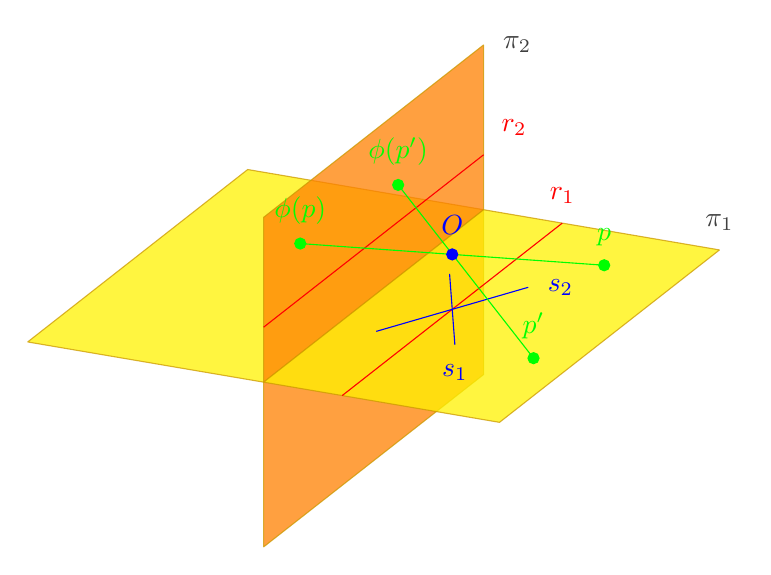
\begin{tikzpicture}
	\begin{axis}[%
	hide axis,
	width=\columnwidth,
	enlargelimits=0.1
	]
	
	\addplot3[patch, patch type=rectangle,opacity=.75,color=yellow]
	coordinates {(0,3,0) (-3,3,0) (-3,-3,0) (0,-3,0)};
	\addplot3[patch, patch type=rectangle,opacity=.75,color=orange]
	coordinates {(0,3,-3) (0,-3,-3) (0,-3,3) (0,3,3)}
	node[label={[black]right:$\pi_2$}]{};
	\addplot3[patch, patch type=rectangle,opacity=.75,color=yellow]
	coordinates {(3,-3,0) (0,-3,0) (0,3,0) (3,3,0)}
	node[label={[black]$\pi_1$}]{};
	
	\addplot3[color=blue,mark=*] coordinates {(1,0,1)}
	node[label=above:{$O$}]{};
	
	\draw [color=red] (axis cs:1,-3,0) -- (axis cs:1,3,0)
	node[label=$r_1$]{};
	\draw [color=red] (axis cs:0,-3,1) -- (axis cs:0,3,1)
	node[label=50:$r_2$]{};
	
	\draw [color=blue] (axis cs:0.5,1,0) -- (axis cs:1.5,-1,0)
	node[label=below:$s_1$]{};
	\draw [color=blue] (axis cs:0.5,-1,0) -- (axis cs:1.5,1,0)
	node[label=right:$s_2$]{};
	
	\addplot3[color=green,mark=*] coordinates {(2,2,0)}
	node[label=$p$]{};
	\addplot3[color=green,mark=*] coordinates {(0,-2,2)}
	node[label=$\phi(p)$]{};
	\draw [color=green] (axis cs:2,2,0) -- (axis cs:0,-2,2);
	
	\addplot3[color=green,mark=*] coordinates {(2.5,-1,0)}
	node[label=$p'$]{};
	\addplot3[color=green,mark=*] coordinates {(0,0.67,1.67)}
	node[label=$\phi(p')$]{};
	\draw [color=green] (axis cs:2.5,-1,0) -- (axis cs:0,0.67,1.67);
	\end{axis}
	\end{tikzpicture}
\end{center}
La idea básica del problema es enviar los puntos de $\pi_1$ a $\pi_2$ mediante la
siguiente aplicación
\[
\begin{aligned}
\phi \colon \pi_1 &\to \pi_2 \\
p &\mapsto \overline{pO} \cap \pi_2
\end{aligned}
\]
\begin{obs}
	\begin{enumerate}[i)]
		\item[]
		\item $\phi$ manda rectas a rectas
		\item\label{item:prob_r1} $\phi$ no esta definida en $r_1$
		\item\label{item:prob_r2} $r_2$ no esta en la imagen de $\phi$
		\item $\phi(s_1)$ y $\phi(s_2)$ son pararelas, por lo tanto, $\phi$ no
		mantiene el paralelismo
		\item $\phi$ no mantiene el tipo de cónica afín
	\end{enumerate}
\end{obs}
Veremos que la solucion para \ref{item:prob_r1} y \ref{item:prob_r2} consistirá
en añadir puntos en el $\infty$.

\subsection{Definición y caracterizaciones del espacio proyectivo}
\begin{defi}
	Sea $\k$ un cuerpo, $\E$ un $\k$-e.v. de $\dim n+1$. El espacio proyectivo asociado a $\E$ es 
	\[\Po (\E) = \setb{\text{s.e.v. de } \dim 1 \text{ de } \E}\]
	Diremos que $\Po (\E)$ tiene dimensión $n$.
\end{defi}
\begin{obs}
	Se cumple $\Po (\E) = (\E \setminus \setb{0}) / \sim$, donde $v \sim v'  \iff \exists \lambda \neq 0, \ v' = \lambda v$ para
	$v, v' \in \E \setminus \setb{0}$.
\end{obs}
\begin{defi}
	Tenemos la siguiente aplicación $\pi$ dada por el paso al cociente.
	\[
	\begin{aligned}
	\pi \colon \E \setminus \setb{0} &\to \Po (\E)\\
	v &\mapsto \pi(v) = [v]\\
	\setb{\text{s.e.v. de } \dim 1 \text{ de } \E} &\leftrightarrow [v]
	\end{aligned}
	\]
\end{defi}
\begin{defi}
	A los elementos de $\Po (\E)$ los llamaremos puntos de $\Po (\E)$.
	\[p = \pi(v) = [v]\]
\end{defi}
\begin{obs}
	\begin{itemize}
		\item[]
		\item Si $\E$ no es relevante, $\Po^n = \Po (\E)$.
		\item Si queremos remarcar $\k$, $\Po_\k^n = \Po (\E)$.
		\item Normalmente $\Po+\k^n = \Po(\k^{n+1}) = (\k^{n+1} \setminus {0})/\sim$.
	\end{itemize}
\end{obs}
\begin{example}
	\begin{enumerate}
		\item []
		\item $\Po^1_{\real}$.
		\begin{center}
		\begin{tikzpicture}
		\begin{axis}[%
		axis equal,
		enlargelimits=0,
		axis lines=center,
		ticks=none,
		ymin=-4,ymax=4,
		xmin=-4,xmax=4
		]
		
		\addplot[color=orange] {2*x};
		\addplot[mark=*,color=orange] coordinates {(1,2)};
		\addplot[color=orange] {0.5*x};
		\addplot[mark=*,color=orange] coordinates {(1,0.5)};
		\addplot[color=orange] {4*x};
		\addplot[mark=*,color=orange] coordinates {(1,4)};
		\addplot[color=orange] {-4*x};
		\addplot[mark=*,color=orange] coordinates {(1,-4)};
		\addplot[color=orange] {-1*x};
		\addplot[mark=*,color=orange] coordinates {(1,-1)};
		\addplot[color=orange] {-0.5*x};
		\addplot[mark=*,color=orange] coordinates {(1,-0.5)};
		\addplot[color=orange] {12*x};
		
		\addplot[mark=*,color=white] coordinates {(0,0)};
		\addplot[mark=o] coordinates {(0,0)};
		
		\draw [color=red] (axis cs:1,-4) -- (axis cs: 1,1)
		node[label=right:$\bb{A}_\real^1$]{};
		\draw [color=red] (axis cs:1,1) -- (axis cs:1,4);
		\end{axis}
		\end{tikzpicture}
		\end{center}
		\item $\Po^2_{\real}$. Ídem.
		\item $\Po^1_{\cx} = (\cx^2 \setminus {0})/\sim \ = \cx \cup \setb{\infty} = S^2$. Las igualdades
		por el momento son por analogía o intuición, más adelante se demostrarán. (Aquí se puede poner un
		dibujo de la proyección estereográfica).
		\item $\Po^2_{\z / 2}$ contiene $7$ puntos pues las rectas de $\z^3$ solo contienen el $0$ y un punto.
	\end{enumerate}
\end{example}
\begin{obs}
	Hemos enunciado la definición algebraica de $\Po_{\real}^{n}$. Existe una definición axiomática que no 
	es igual en algunos casos patológicos.
\end{obs}
\subsection{Variedades lineales proyectivas}
\begin{defi}
	Sea $\E$ un $\k$-e.v. de dimensión $n+1$, sea $\Po^n = \Po(\E)$.
	Llamaremos variedad lineal (proyectiva) de dimensión $r$ a cualquier conjunto 
	de la forma:
	\[V = \pi(H \setminus \setb{0})\]
	donde $H \subseteq \E$ es un subespacio vectorial de dimensión $r+1$.
	
	Por convención defnimos la siguiente notación:
	\[V = \pi(H \setminus \setb{0}) = \pi(H)\]         
\end{defi}    
\begin{example}
	\begin{itemize}
		\item []
		\item $\Po^n = \pi(\E)$ es una variedad lineal de dimensión $n$.
		\item $p \in \Po^n$, $p = \pi(v) = \pi([v])$ es una varidead lineal de dimensión $0$.
		\item $\emptyset = \pi({\emptyset_{\E}})$ es una variedad lineal de dimensión $-1$.
	\end{itemize}
\end{example}
\begin{defi}
	\begin{itemize}
		\item []
		\item $\dim V = 1 \longrightarrow$ Recta
		\item $\dim V = 2 \longrightarrow$ Plano
		\item $\dim V = n-1 \longrightarrow$ Hiperplano
	\end{itemize}
\end{defi}
\begin{lema}
	$V = \pi(H\setminus\setb{0}) \iff H \setminus \setb{0} = \pi^{-1}(V)$
\end{lema}
\begin{ej}
	Demostrar el lema anterior.
\end{ej}
\begin{obs}
	Hay una biyección
	\[\setb{\text{s.e.v. de } \E}
	\mathrel{\mathop{\rightleftarrows}^{\mathrm{\pi}}_{\mathrm{\pi^{-1}}}}
	\setb{\text{variedades lineales de } \Po(\E)}\]
	\begin{itemize}
		\item con dimension $r+1 \leftrightarrow r$
		\item $H_1 \subseteq H_2 \iff V_1 \subseteq V_2$ con $V_i=\pi(H_i)$
		\item Las operaciones $+$ y $\cap$ definidas para subespacios, se definen
		a traves de esta biyección a variedades.
	\end{itemize}
\end{obs}
